% document formatting
\documentclass[10pt]{article}
\usepackage[utf8]{inputenc}
\usepackage[left=1in,right=1in,top=1in,bottom=1in]{geometry}
\usepackage[T1]{fontenc}
\usepackage{xcolor}

% math symbols, etc.
\usepackage{amsmath, amsfonts, amssymb, amsthm}

% lists
\usepackage{enumerate}
\usepackage{tabularx}
\usepackage{multicol}
\usepackage[table,xcdraw]{xcolor}

% images
\usepackage{graphicx} % for images

% code blocks
\usepackage{minted, listings} 

% verbatim greek
\usepackage{alphabeta}

\graphicspath{{./assets/images/Week 3}}

\newcommand{\solution}{\textbf{Solution:}} 
\newcommand{\example}{\textbf{Example: }}
\newcommand{\water}{\text{H$_2$O}}
\newcommand{\hydroxide}{\text{OH$^-$}}
\newcommand{\hydronium}{\text{H$_3$O$^+$}}
\newcommand{\proton}{\text{H$^+$}}
\newcommand{\pc}{$^+$}
\newcommand{\nc}{$^-$}
\newcommand{\ka}{\text{$K_\text{a}$}}

\title{CHEM 153A Week 3}

\author{Aidan Jan}
\date{\today}

\begin{document}
\maketitle
\section*{Protein Folding Continued}
\subsection*{More Questions - Levinthal's Paradox}
\begin{itemize}
    \item Other experiments like Anfinsen's raised more questions
    \begin{itemize}
        \item Denatured proteins refold in 0.1-1000 seconds
        \item Take a hypothetical protein with 100 amino acids
        \item Due to allowed rotations, amino acids can have 3 conformations
        \item That's roughly $3^{100}$ possibilities ($\approx 5 \times 10^{47}$)
    \end{itemize}
    \item If the protein can visit one conformation every picosecond ($10^{-12}$ s), searching every possibility would take $5 \times 10^{47} \times 10^{-12}$ seconds, or $1.6 \times 10^{28}$ years.
    \item This is the left diagram
\end{itemize}
\begin{center}
    \includegraphics*[width=\textwidth]{L1_1.png}
\end{center}
\subsection*{The Thermodynamics of Protein Folding}
\begin{itemize}
    \item Free Energy Funnel:
    \begin{itemize}
        \item Unfolded states have high degree of conformational entropy, thus there is high free energy.
        \item The free energy funnel shows that the closer the protein is to its \textbf{native state}, the ideal, lowest energy, folded form, the lower energy it has.
        \begin{itemize}
            \item The middle diagram suggests that there is a pathway guiding the protein folding to the lowest energy state.  This is on the right track, but is not correct.
            \item The right diagram states there are multiple stable intermediates leading to the final folded protein.  This is the most accurate diagram.
        \end{itemize}
    \end{itemize}
\end{itemize}

\subsection*{Hydrophobic Collapse $\rightarrow$ Molten Globule}
\textbf{Hydrophobic collapse} is the rapid burying of hydrophobic residues in the center of the protein - they want to escape their watery environment.
\begin{itemize}
    \item e.g., Val, Leu, Ile, etc.
    \begin{center}
        \includegraphics*[width=\textwidth]{L1_2.png}
    \end{center}
    \item Hydrophobic collapse is entropy-driven: water molecules become more ordered around hydrophobic residues, and the collapse releases that ordered water, increasing entropy.
\end{itemize}
\begin{center}
    \includegraphics*[width=\textwidth]{L1_3.png}
\end{center}
\begin{itemize}
    \item This collapse forms the \textbf{molten globule}, an intermediate transitioning to the final form of the protein
\end{itemize}
\begin{center}
    $\boxed{\includegraphics*[scale=0.5]{L1_4.png}}$
    $\boxed{\includegraphics*[scale=0.35]{L1_5.png}}$
\end{center}
\subsection*{Protein Folding and Energy Landscape}
\begin{center}
    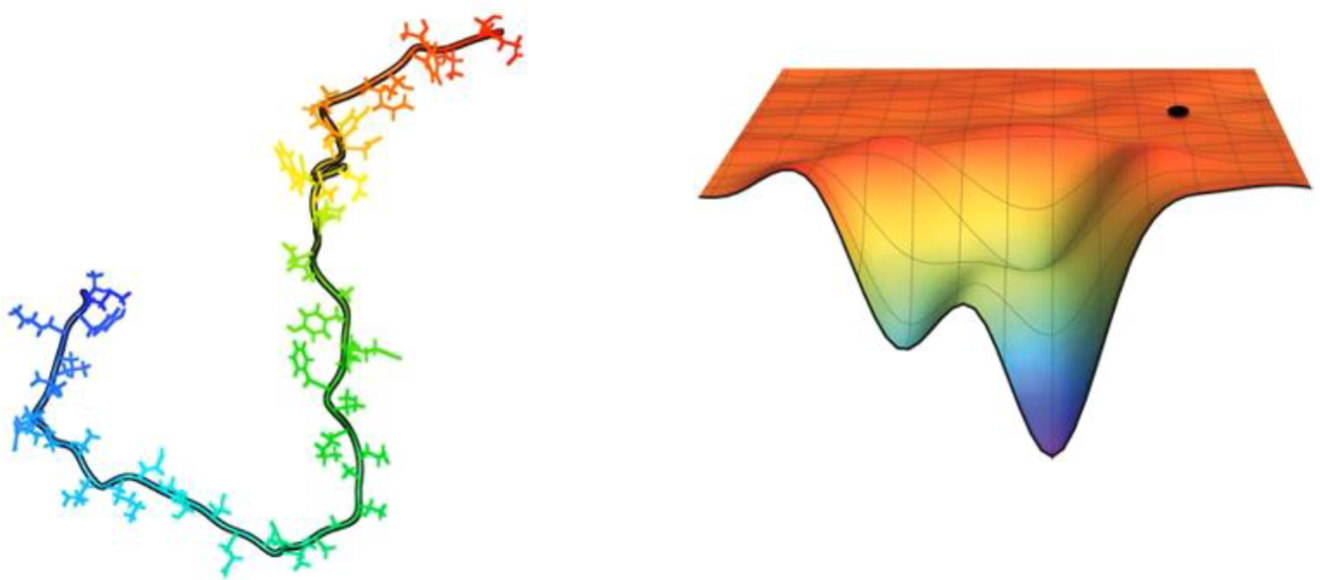
\includegraphics[width=\textwidth]{L1_6.png}
\end{center}
\subsection*{Other Significant Factors in Protein Folding}
\begin{itemize}
    \item \textbf{\underline{Chain conformational entropy}} is the entropy \textit{decrease} due to the formation of an ordered polypeptide
    \item \textbf{\underline{Hydrogen bonding}} serves an important role, mediating interactions with the surrounding water as well as connecting the outer surface of the protein with the hydrophobic core
    \begin{itemize}
        \item They also stabilize interactions between peptide chains (secondary structure)
        \item Enthalpy decrease
    \end{itemize}
    \item \textbf{\underline{London dispersion forces}} hold together the hydrophobic core (enthalpy decrease)
    \item \textbf{\underline{Electrostatic forces}} can form between charged R groups (enthalpy decrease)
\end{itemize}

\subsection*{Protein folding is enthalpically driven}
Although folding a protein reduces its entropy, the process is driven by the \textbf{enthalpy gain} from forming stabilizing interactions.  These forces - hydrogen bonding, van der Waals interactions, and electrostatic forces - make folding energetically favorable, leading to a stable, functional protein.
\begin{itemize}
    \item \textbf{Conclusion:} Protein folding is \textbf{enthalpically favorable} ($\Delta H < 0$) but \textbf{entropically unfavorable} ($\Delta S < 0$)
\end{itemize}
\begin{center}
    \includegraphics*[width=\textwidth]{L1_7.png}
\end{center}

\subsection*{Summary of protein folding}
\begin{itemize}
    \item Unfolded protein rapidly collapses (hydrophobic collapse) to increase entropy of surrounding water
    \item Molten globule state(s) form, with some early secondary structure
    \begin{itemize}
        \item Serves as pre-folded state, serving to constrain energetic possibilities
        \item \textbf{"Cooperative" effect} emerges, once one interaction forms, the next interaction is easier to form
    \end{itemize}
    \item Molten globule state then slowly works its way to the final native structure.
\end{itemize}
\begin{center}
    \includegraphics*[scale=0.5]{L1_8.png}
    \includegraphics*[scale=0.5]{L1_9.png}
\end{center}


\section*{Protein Structures}
\begin{itemize}
    \item \textbf{Protein segments can adopt regular secondary structures such as the $\alpha$ helix and the $\beta$ conformation.}
    \item These structures are defined by particular values of $\phi$ and $\psi$ and their formation is impacted by the amino acid composition on their segment.
    \item All of the $\phi$ and $\psi$ values for a given protein structure can be visualized using a Ramachandran plot.
\end{itemize}

\subsection*{Protein Secondary Structure}
\begin{itemize}
    \item \textbf{secondary structure =} describes the spatial arrangement of the main-chain atoms in a segment of a polypeptide chain
    \begin{itemize}
        \item \textit{regular} secondary structure = $\phi$ and $\psi$ remain the same throughout the segment
        \item common types = $\alpha$ helix, $\beta$ conformation, $\beta$ turn, random coils
    \end{itemize}
\end{itemize}
\begin{center}
    \includegraphics*[width=\textwidth]{L2_1.png}
\end{center}

\subsubsection*{The $\alpha$ Helix is a Common Protein Secondary Structure}
\begin{itemize}
    \item $\alpha$ helix = simplest arrangement, maximum number of hydrogen bonds
    \begin{itemize}
        \item backbone wound around an imaginary longitudinal axis
        \item R groups protrude out from the backbone
        \item Each helical turn = 3.5 residues, $\sim$5.4 \r{A}
    \end{itemize}
\end{itemize}
\begin{center}
    \includegraphics*[scale=0.4]{L2_2.png}
\end{center}

\subsection*{Dihedral Angles Define Protein Conformations}
The following table shows idealized $\phi$ and $\psi$ angles for common secondary structures in proteins
\begin{center}
\begin{tabular}{lcc}
\rowcolor[HTML]{D0E7D2} 
\textbf{Structure}                                    & $\phi$                            & $\psi$                            \\ \hline
\multicolumn{1}{|l|}{$\alpha$ Helix}                  & \multicolumn{1}{c|}{$-57^\circ$}  & \multicolumn{1}{c|}{$-47^\circ$}  \\ \hline
\multicolumn{1}{|l|}{Conformation: Antiparallel}      & \multicolumn{1}{c|}{$-139^\circ$} & \multicolumn{1}{c|}{$+135^\circ$} \\ \hline
\multicolumn{1}{|l|}{$\beta$ Conformation: Parallel}  & \multicolumn{1}{c|}{$-119^\circ$} & \multicolumn{1}{c|}{$+113^\circ$} \\ \hline
\multicolumn{1}{|l|}{Collagen triple helix}           & \multicolumn{1}{c|}{$-51^\circ$}  & \multicolumn{1}{c|}{$+153^\circ$} \\ \hline
\multicolumn{1}{|l|}{$\beta$ Turn type I: $i + 1$}    & \multicolumn{1}{c|}{$-60^\circ$}  & \multicolumn{1}{c|}{$-30^\circ$}  \\ \hline
\multicolumn{1}{|l|}{$\beta$ Turn type I: $i + 2$}    & \multicolumn{1}{c|}{$-90^\circ$}  & \multicolumn{1}{c|}{$0^\circ$}    \\ \hline
\multicolumn{1}{|l|}{$\beta$ Turn type II: $i + 1$}   & \multicolumn{1}{c|}{$-60^\circ$}  & \multicolumn{1}{c|}{$+120^\circ$} \\ \hline
\multicolumn{1}{|l|}{$\beta$ Turn type II: $i + 2$}   & \multicolumn{1}{c|}{$+80^\circ$}  & \multicolumn{1}{c|}{$0^\circ$}    \\ \hline
\end{tabular}
\end{center}

\subsection*{Handedness of the $\alpha$ Helix}
\begin{itemize}
    \item Right-handed:
    \begin{itemize}
        \item R groups protruding away from the helical backbone
        \item most common
    \end{itemize}
    \item extended left-handed: theoretically less stable, not observed in proteins
\end{itemize}

\begin{center}
    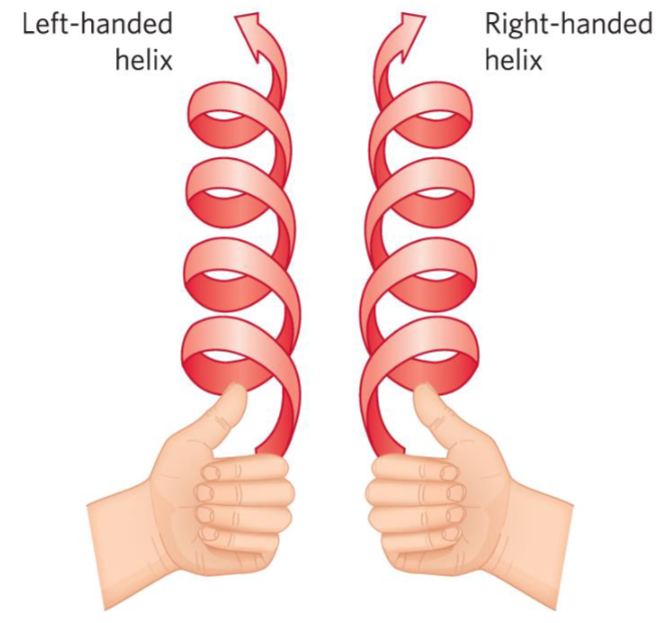
\includegraphics[scale=0.4]{L2_3.png}
    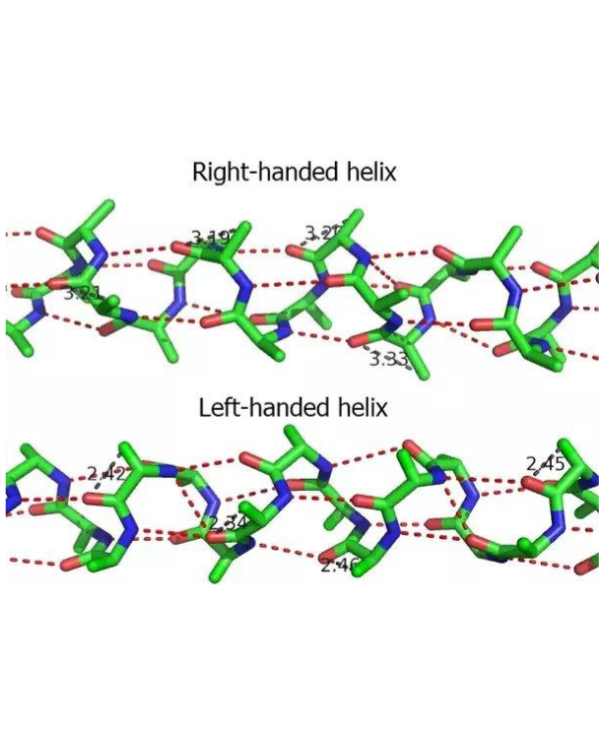
\includegraphics[scale=0.4]{L2_4.png}
\end{center}

\subsection*{Intrahelical Hydrogen Bonds}
\begin{itemize}
    \item Between hydrogen atom attached to the electronegative nitrogen atom of residue $n$ and the electronegative carbonyl oxygen atom of residue $n + 4$
    \item Confers significant stability
\end{itemize}

\subsection*{Amino Acid Sequence Affects Stability of the $\alpha$ Helix}
\begin{itemize}
    \item amino acid residues have an intrisic propensity to form an $\alpha$ helix
    \item $\alpha$ helix = simplest arrangement, maximum number of hydrogen bonds
    \begin{itemize}
        \item backbone wound around an imaginary longitudinal axis
        \item R groups protrude out from the backbone
        \item each helical turn = 3.6 residues, ~5.4 \r{A}
    \end{itemize}
    \item Interactions between R chains spaced 3-4 residues apart can stabilize or destabilize $\alpha$ helix
    \begin{itemize}
        \item charge, size, and shape of R chains can destabilize
        \item formation of ion pairs and hydrophobic effect can stabilize
    \end{itemize}
\end{itemize}
\begin{center}
    \includegraphics*[scale=0.7]{L2_5.png}
\end{center}
\subsection*{Amphipathic $\alpha$-helices}
Can be found at the surface of a water-soluble globular protein, whereas hydrophobic helices are on the inside.
\begin{itemize}
    \item As the name implies, an \textbf{amphipathic (or amphiphilic) helix is an $\alpha$-helix with both hydrophobic and hydrophilic amino acid residues} arranged in such a way as to create two faces on opposite sides of the helix, one face being hydrophobic.
    \item An example is the bottom left image above (yellow is nonpolar, green is polar)
\end{itemize}
\subsubsection*{Proline and Glycine Occur Infrequently in an $\alpha$ Helix}
\begin{itemize}
    \item Proline = introduces destabilizing kink in helix
    \begin{itemize}
        \item Nitrogen atom is part of rigid ring
        \item rotation about N-C$_\alpha$ bond not possible
    \end{itemize}
    \item Glycine = high conformational flexibility, takes up coiled structures.
\end{itemize}

\subsubsection*{Amino Acid Residues Near the End of a $\alpha$ Helix Segment Affect Stability}
\begin{itemize}
    \item small electric dipoles in each peptide bond align through hydrogen bonds
    \item negativevly charged amino acids often found near the NH$_3^+$ terminus
    \item positively charged amino acid often found near the COO$^-$ terminus
\end{itemize}
\begin{center}
    \includegraphics*[scale=0.6]{L4_1.png}
\end{center}

\subsection*{The $\beta$ Conformation Organize Polypeptide Chains into Sheets}
\begin{itemize}
    \item \textbf{$\beta$ conformation} = backbone extends into a zigzag
    \begin{itemize}
        \item $\beta$ strand = single protein segment
        \item $\beta$ sheet = several strands in $\beta$ conformation side by side
    \end{itemize}
\end{itemize}
\begin{center}
    \includegraphics*[width=\textwidth]{L4_2.png}
\end{center}

\subsubsection*{Adjacent Polypeptide Chains in a $\beta$ Sheet Can Be Antiparallel or Parallel}
\begin{itemize}
    \item antiparallel = opposite orientation  (occur more frequently)
    \item parallel = same orientation
    \item H bonds form between backbone atoms of adjacent segments
\end{itemize}
\begin{center}
    \includegraphics*[scale=0.7]{L4_3.png}
\end{center}

\subsubsection*{$\beta$ Turns are Common in Proteins}
\begin{itemize}
    \item $\beta$ turns = connect ends of two adjacent segments of an \underline{antiparallel} $\beta$ sheet
    \begin{itemize}
        \item 180$^\circ$ turn
        \item involves 4 residues
        \item hydrogen bond forms between first and fourth residue
        \item Gly (residue 2) and Pro (residue 3) often occur in $\beta$ turns.
    \end{itemize}
\end{itemize}
\begin{center}
    \includegraphics*[width=\textwidth]{L4_4.png}
\end{center}

\subsubsection*{Notes on determining parallel vs antiparallel $\beta$ sheets}
\begin{center}
    \includegraphics*[width=\textwidth]{L4_5.png}
\end{center}
Red labels carbonyl oxygens while blue labels the amine nitrogens

\subsection*{Common Secondary Structures Have Characteristic Dihedral Angles}
\begin{itemize}
    \item dihedral angles $\varphi$ (phi) and $\psi$ (psi) associated with each residue \underline{completely} describe secondary structure
    \item \textbf{Ramachandran plots:}
    \begin{itemize}
        \item visualize all $\varphi$ and $\psi$ angles
        \item test quality of three-dimensional protein structures
    \end{itemize}
\end{itemize}
\begin{center}
    \includegraphics*[scale=0.5]{L4_6.png}
\end{center}
\subsection*{Ramachandran Plot - Glycine}
\begin{itemize}
    \item Glycine falls frequently outside the expected ranges.
\end{itemize}
\begin{center}
    \includegraphics*[width=\textwidth]{L4_7.png}
    \includegraphics*[scale=0.7]{L4_8.png}
\end{center}
\begin{itemize}
    \item Due to the minimal bulk, glycine residues have far more conformational flexibility than other amino acid residues
    \begin{itemize}
        \item Actually works against it, destabilizes $\alpha$ and $\beta$
    \end{itemize}
    \item This is why its Ramachandran is so well populated
    \item This is also why glycine is often found in \textbf{loop regions} of the protein structure (polypeptide taking a turn)
\end{itemize}
\subsection*{Ramachandron Plot - Proline}
\begin{itemize}
    \item Due to its R-group ring structure, proline is highly constrained and can only adopt specific angles
    \item Not likely to show up in either $\beta$ sheets or $\alpha$ helices (destabilizes both, creating kinks)
\end{itemize}
\begin{center}
    \includegraphics*[width=\textwidth]{L4_9.png}
\end{center}

\pagebreak
\section*{Protein Tertiary and Quaternary Structures}
Tertiary structure describes the well-defined, three-dimensional fold adopted by a protein.
\begin{center}
    \textbf{Shape $\longrightarrow$ Function}
\end{center}
\begin{itemize}
    \item \textbf{tertiary structure} = overall three-dimensional arrangement of all the atoms in a protein
    \begin{itemize}
        \item weak interactions and covalent bonds hold interactng segments in position
    \end{itemize}
    \item \textbf{quaternary structure} = arrangement of 2+ separate polypeptide chains in three-dimensional complexes
\end{itemize}


\end{document}